\section{区块链搜索引擎}
\label{sec:search}

\subsection{简介}

随着越来越多的智能合约被开发者部署,用户面对海量的智能合约,搜索的需求也变得突出起来。智能合约仅仅是代码,并不包含任何功能描述,很难利用搜索引擎技术为智能合约建立索引。我们将用多种手段为智能合约建立合适的索引:
\begin{itemize}
	\item 爬取智能合约相关网页资料,为其和区块链智能合约建立映射关系;
	\item 鼓励开发者上传验证过的智能合约源代码,分析其代码功能和语义,为源代码建立索引,提供相似合约搜索;未提供源代码的智能合约,进行反编译得到其源代码;
	\item 为智能合约建立规范,任何符合此规范的智能合约,都能被检索并被用户搜索到,鼓励开发者在创建智能合约时,提供合约信息描述。 \\

	\begin{figure}[ht]
  	\centering
  	\begin{minipage}{.4\linewidth}
	\begin{lstlisting}[frame=single]
contract SearchableContract {
   string public language;
   string public author;
   string public name;
   string public title;
   string public description;
   string public tags;
}
	\end{lstlisting}
  	\end{minipage}
	\end{figure}

\end{itemize}

\subsection{搜索基础架构}

我们认为,搜索服务为了提供最佳的用户体验,中心化的架构更为适合。星云链开发组将实现一个搜索服务,实时检索所有智能合约,做多语言的分词,建立全文索引,最终提供一个友好的Web界面给用户使用。\textbf{NR排名算法的公正性和每个节点的可验证性保证了中心化搜索服务的公正性},所有搜索后台代码都将开源给社区。第三方开发者也可据此创建独立的搜索服务。搜索服务架构如图\ref{fig:search-arch}所示。

\begin{figure}[h]
\centering
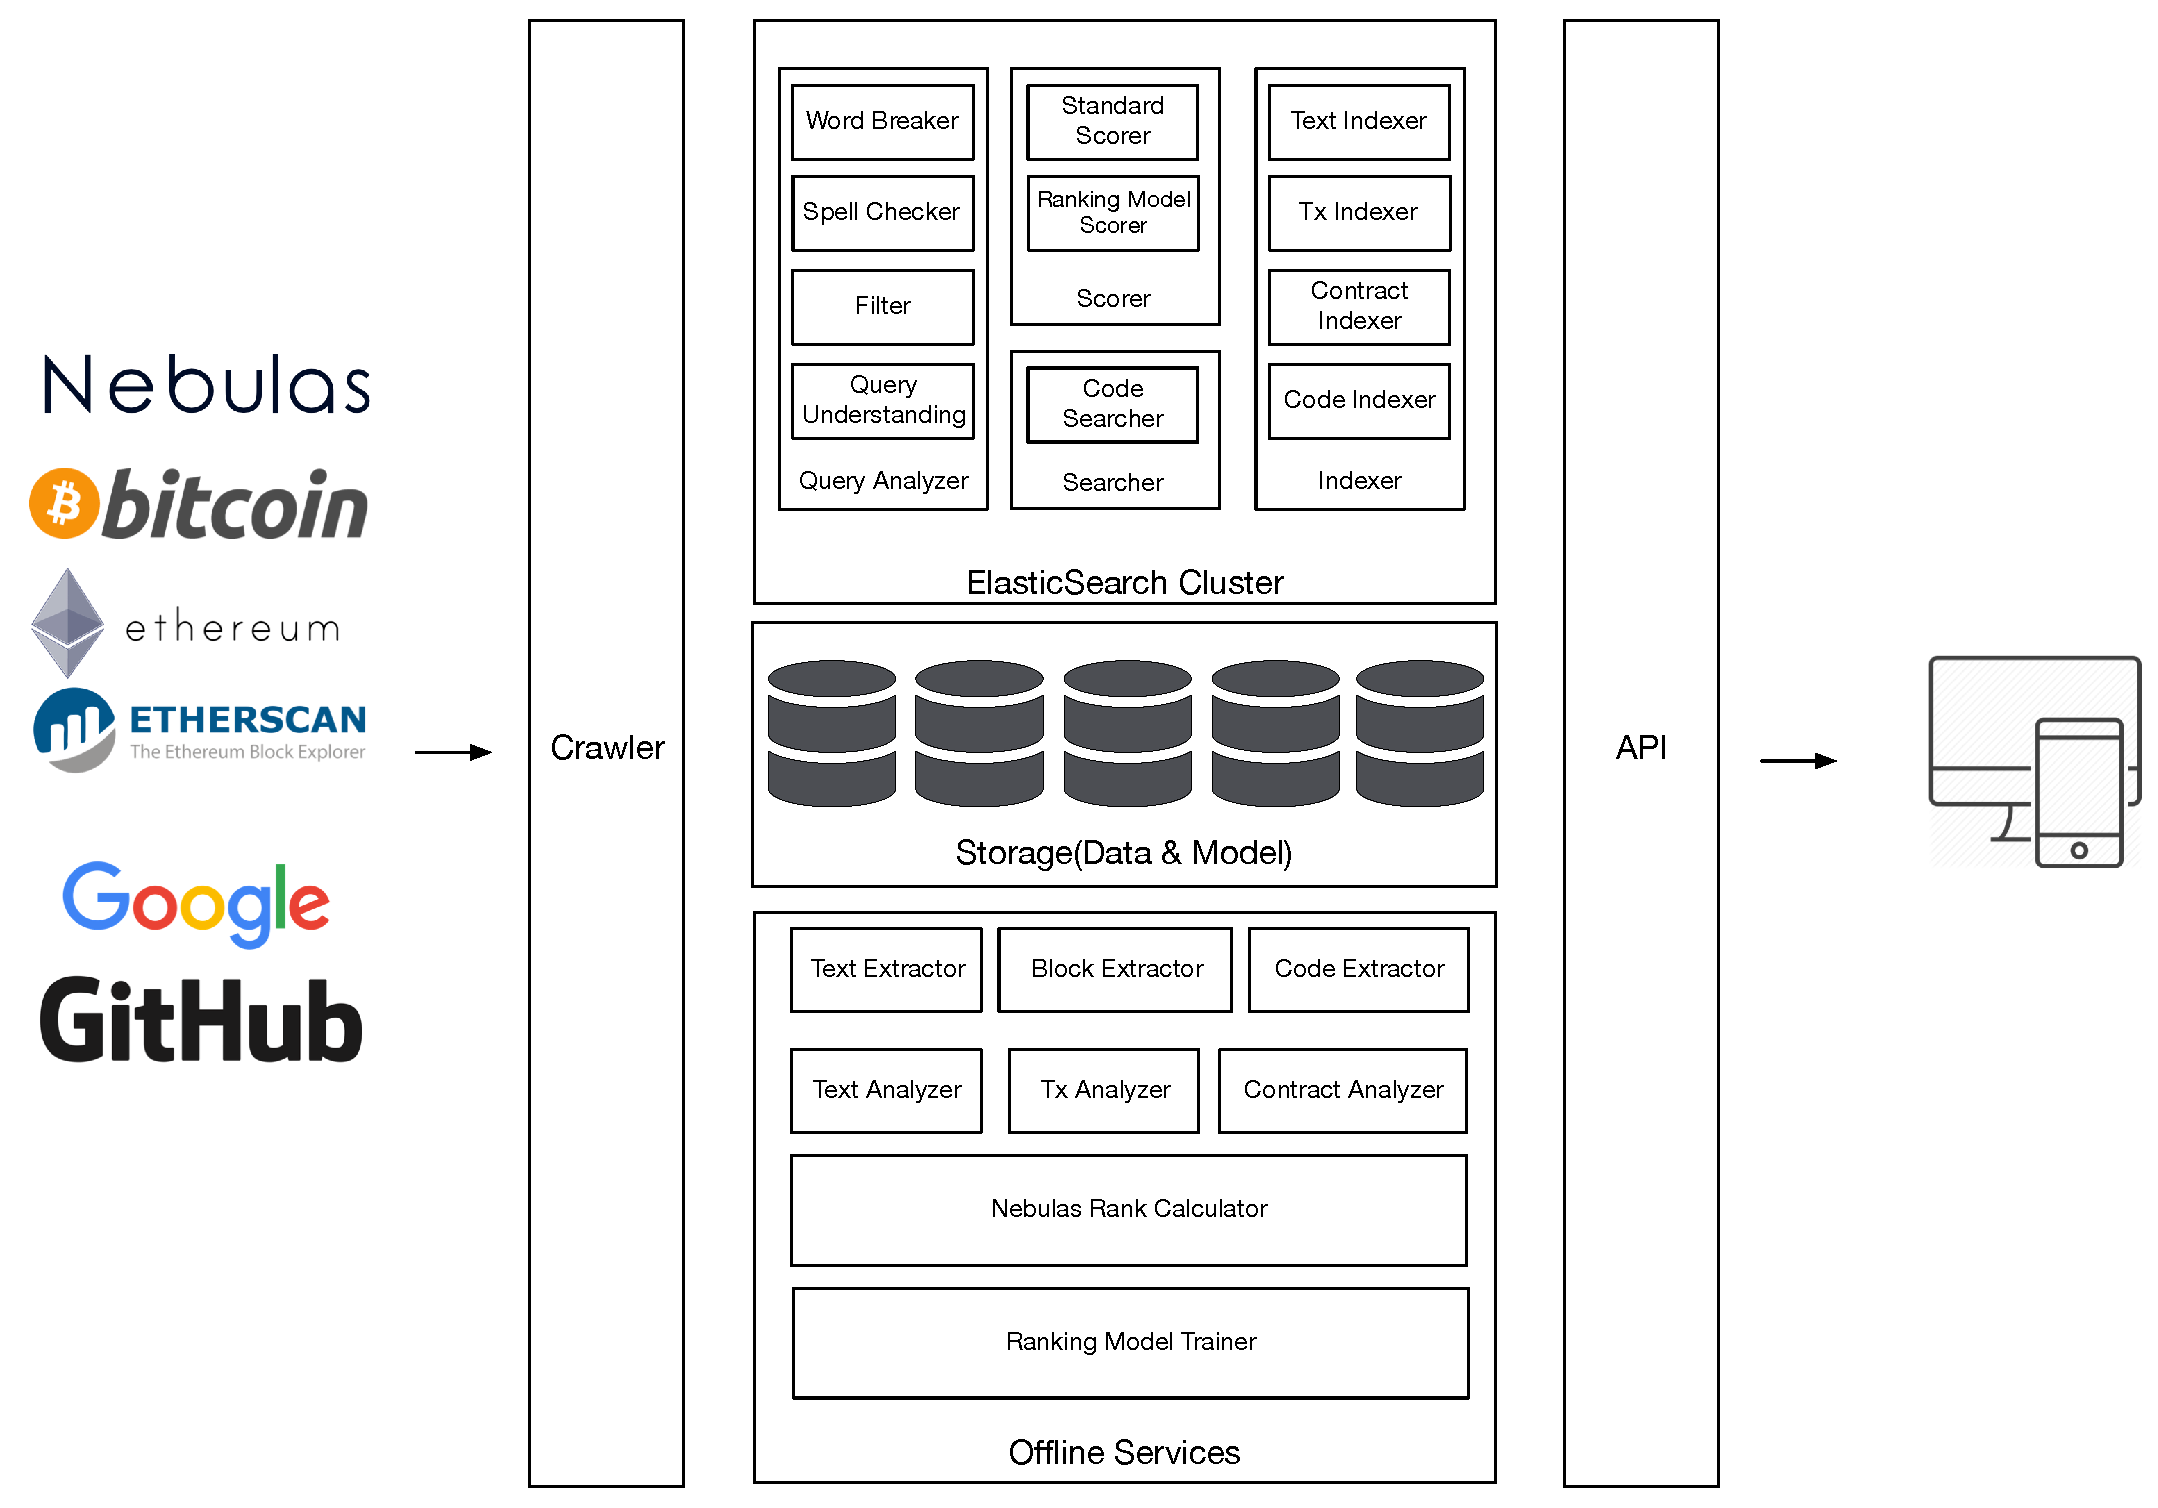
\includegraphics[width=16cm]{./figs/search-arch-new}
\caption{搜索服务架构}
\label{fig:search-arch}
\end{figure}

\begin{itemize}
	\item \textbf{Crawler} 区块链搜索引擎爬虫数据源分为两种,一种从区块链上收集区块信息和智能合约代码等信息,一种从公开网址上爬取智能合约相关资料,包括介绍、Dapp用户评论、新闻资讯等。
	\item \textbf{Extractor} 包括Text Extractor, Block Extractor和Code Extractor,分别提供文本信息、区块信息和智能合约代码提取服务。
	\item \textbf{Analyzer} 包括Text Analyzer, Tx Analyzer, Contract Analyzer,分别为文本信息、区块交易信息和智能合约分析器,其中智能合约分析器包括合约反编译、源代码功能、语义分析,网页解析等。
	\item \textbf{Nebulas Rank Calculator} 星云指数计算服务,离线计算每个非合约账户和合约账户的星云指数。
	\item \textbf{Ranking Model Trainer} 排序模型训练。考虑到交易Graph,排序规则考虑了多个因素:匹配字段,文本相关度,合约的NR Rank值,合约的交易数量、频度和深度,与合约发生交易的用户NR Rank值,合约安全性等等。我们根据用户的实际使用情况,用机器学习算法(GBDT、人工神经网络都是候选)训练排序打分模型,根据用户的反馈不断优化。训练后的模型被搜索服务的Scorer使用。
	\item \textbf{Query Analyzer} 关键词分析服务,包括多语言分词器Word Breaker,拼写检查器Spell Checker等。
	\item \textbf{Indexer} 从Analyzer中建立合适的索引,支持全量和增量索引。
	\item \textbf{Scorer} 分为两个level:Level-1 Standard Scorer从ElasticSearch中召回候选结果集,目标是尽可能把潜在的候选结果,在ElasticSearch集群中通过快速有效的排序打分召回,Level-1召回的结果数量有限,控制在几千以内;Level-2 Ranking Model Scorer使用 Offline Rank Model,计算每个Level-1结果候选集的得分,重新排序,这个结果较为精确,可以直接给用户使用。
	\item \textbf{Searcher} 负责和ElasticSearch集群通信,以及对搜索结果包装返回给搜索前端。
	\item \textbf{API} 对外提供完善的搜索API服务。
	\item \textbf{ElasticSearch Cluster} ES服务器集群。星云链团队考虑使用开源搜索引擎ElasticSearch作为其全文索引支持。
\end{itemize}

\subsection{趋势榜单}
星云链将结合星云指数构建趋势榜单,提供给用户可视化的区块链多维度价值。
\begin{itemize}
\item \textbf{非合约账户Nebulas Rank榜单}~~呈现每日NR榜单,以及NR快速提升和快速下降榜单,并且可视化呈现各个账户的R变化趋势,以及整个网络健康程度变化趋势。
\item \textbf{合约账户Nebulas Rank榜单}~~根据非合约账户NR值,计算合约账户的NR榜单,以及快速提升和快速下降榜单,各个合约的变化趋势,以及整个网络智能合约数量和使用频次的趋势图。除此之外,我们还将呈现不同领域的智能合约榜单,比如Token合约榜单、预测市场合约榜单等等,以展示更多维度的信息。
\item \textbf{智能合约开发者榜单}~~根据合约账户榜单,计算合约开发者的贡献度榜单,以及贡献度快速提升榜单,展示优秀合约开发者及其应用。
\end{itemize}

\subsection{关键词搜索}
用户提供关键词,描述智能合约的标题、作者、功能等文本信息,在海量的智能合约中找到匹配的合约。对于文本搜索,目前有非常成熟的算法和技术,基于自然语言处理和倒排索引技术,我们可以在海量的智能合约索引库里高效的检索和排序。关键的技术如下:

\begin{enumerate}
	\item 面向主题的分布式爬虫技术
	\item 多语言分词技术:对于西文词汇,分词较为简单。对于中文分词,有多种算法可进行分词:正向最大匹配,逆向最大匹配,最短路径分词,统计分词等;
	\item 查询词纠错、语义理解
	\item 倒排索引,分布式搜索架构
	\item 排序算法,给搜索结果排序
\end{enumerate}

其中排序算法将结合Nebulas Rank来设计,我们把区块链世界中用户之间的转账类比互联网世界的网页引用关系,构建出区块链交易图,然后利用\ref{subsec:leaderrank}中提出的NR排名算法,计算非合约用户的NR排名,然后结合\ref{dip:arith}中介绍的合约排名算法,计算合约的排名结果,最后应用于搜索结果排序。


\subsection{相似智能合约搜索}
开发者和某些用户,可能有根据合约代码片段,搜索具有相似功能的智能合约的需求。不同于普通的关键词搜索,代码相似度有其特殊性。我们需要有一定的算法,通过数值或者百分比的形式对代码相似度进行度量,从而提供相似智能合约搜索的功能。

目前学术界对代码相似度算法主要有字符串编辑距离、Token序列相似度、抽象语法树相似度和程序依赖图相似度四个流派,他们分别从不同维度描述了代码文本、结构和语法上的相似度,我们结合主流4个流派的思路,提出了星云链合约代码相似度算法的12种特征,如Skeleton Tree、Type Signature和Libaray Calls等,详情见附录\ref{appendix:sim_code}。

相似智能合约搜索结果,和关键词搜索结果一样,使用同样的合约排名算法排序,给出最终结果。
